\documentclass{beamer}
%\usepackage[usenames,dvipsnames]{xcolor}

\usepackage{_defsAndPackages675notation}
\usepackage{_defsAndPackages675beamer}

\begin{document}

\title{\alg{Linear Methods for Regression: Introduction}}
\subtitle{\classTitle}
%\author{\alg{Darren Homrighausen, PhD}}
%\institute{\classTitle}
\date{}



\begin{frame}
\maketitle
%\titlepage
%\begin{figure}[h!]
%  \centering
%  \includegraphics[width=1in]{.../figures/CSU_logo2.eps}
%\end{figure}
%
\organization
%
\end{frame}

\begin{frame}
\frametitle{The Setup}
Suppose we have data 
\[
\data = \{ (X_1 , Y_1), (X_2 , Y_2), \ldots, (X_n , Y_n) \},
\]
where 
\begin{itemize}
	\item $X_i \in \mathbb{R}^p$  are the \alg{features} 

	{\scriptsize (or \alg{explanatory variables} or \alg{predictors} or \alg{covariates}.  NOT INDEPENDENT VARIABLES!)}
\item $Y_i \in \mathbb{R}$ are the \alg{response} variables.

	{\scriptsize (NOT DEPENDENT VARIABLE!)}
\end{itemize}
\vsp

Our goal for this class is to find a way to explain (at least approximately) the \alo{relationship}
between $X$ and $Y$.
\vsp
\end{frame}

\begin{frame}
\frametitle{Prediction risk for regression}
Given the \alo{training data} $\data$, we want to predict some independent \alo{test data} $Z = (X,Y)$

\vsp
This means forming a $\hat f$, which is a function of both the range of $X$ and the training data $\data$, 
which provides predictions $\hat Y = \hat f(X)$.

\vsp
The quality of this prediction is measured via the prediction risk\footnote{ Note: sometimes we integrate with
respect to $\data$ only, $Z$ only, neither (loss), or both.}
\[
R(\hat{f}) = \P_{\data,Z}(Y - \hat{f}(X))^2.
\]

We know that the \alo{regression function}, $f_*(X) = \P[Y | X]$, is the best possible predictor.  


\vsp
Note that $f_*$ is {\it unknown}
\end{frame}
%
%\begin{frame}
%\frametitle{Prediction risk for regression}
%Note that $R(\hat{f})$ can be written as
%\[
%R(\hat{f}) = \int \textrm{bias}^2(x) d\P_X + \int \textrm{var}(x) d\P_X + \sigma^2
%\]
%where
%\begin{align*}
%\textrm{bias}(x) & = \P\hat{f}(x) - f_*(x)\\
%\textrm{var}(x) & = \V\hat{f}(x) \\
%\sigma^2 & = \P(Y - f_*(X))^2
%\end{align*}
%\end{frame}


\begin{frame}
\frametitle{Notation recap}
\begin{itemize}
\item $X$ is a vector of \alg{measurements} for each subject

\script{Example: $X_i = [1, \textrm{income}_i, \textrm{education}_i]^{\top}$}
\item $x$ is a vector of \alg{subjects} for each measurement

\script{Example: $x_j = [\textrm{income}_1, \textrm{income}_2, \ldots,\textrm{income}_n]^{\top}$}
\item $X_i^j$ is the $j^{th}$ measurement on the $i^{th}$ subject

\script{Example: $X_i^j = \textrm{income}_i$}
\end{itemize}
\end{frame}


\transitionSlide{Imposing linearity}



\begin{frame}
\frametitle{A linear model: Multiple regression}
If we specify the model: $f_*(X) = X^{\top}\beta =  \sum_{j=1}^p x_j \beta_j$ 
\[
\Rightarrow Y_i = X_i^{\top}\beta + \epsilon_i
\] 
 Then we recover the usual linear regression formulation
\[
\X = 
\left[
\begin{array}{ccc}
x_1 & \cdots & x_p 
\end{array}
\right]
=
\left[
\begin{array}{cccc}
X_{1}^{\top} \\
X_{2}^{\top} \\
\vdots    \\
X_{n}^{\top} \\
\end{array}
\right].
\]
\script{When referring to $j^{th}$ entry of any $X_i$, we write $X_i^j$}
\vsp

Commonly, a column $x_0^{\top} = \underbrace{(1,\ldots,1)}_{n \textrm{ times}}$ is included

This encodes an intercept term, with intercept parameter $\beta_0$ 

\vsp

We could (should?) seek to find a $\beta$ such that $Y \approx \X\beta$

\end{frame}

\begin{frame}
\frametitle{A linear model: Polynomial effects}
Instead, we may believe 
\[
f_*(X) = \beta_0 + \sum_{j=1}^p X^j \beta_j + \sum_{j=1}^p \sum_{j'=1}^p X^jX^{j'} \alpha_{j,j'}
\]
 Then the \alo{feature} matrix is
\[
\X = 
\left[
\begin{array}{cccccccc}
x_0 & x_1 & \cdots & x_p & x_1^2 & x_1x_2 & \cdots & x_p^2
\end{array}
\right]
\]
\script{Here, interpret vector multiplication in the entrywise sense, as in \alr{R}: {\tt x * y}} 

\end{frame}


\begin{frame}
\frametitle{A linear model: General form}
Specify 
%\footnote{We'll revisit this later with Projection Pursuit/Neural Nets.} 
functions $\phi_k:\R^p \rightarrow \R$, $k=1,\ldots,K$

\[
\X = 
\left[
\phi_k(X_i)
\right]
=
\left[
\begin{array}{c}
\Phi(X_{1})^{\top} \\
\Phi(X_{2})^{\top} \\
\vdots    \\
\Phi(X_{n})^{\top} \\
\end{array}
\right]
 \in R^{n\times K},
\]
where $\Phi(\cdot)^{\top} = (\phi_1(\cdot), \ldots, \phi_K(\cdot))$.

\vsp
\smallCapGreen{Example: }
\[
\phi_k(X) = X^jX^{j'}
\]
is an interaction for the $j^{th}$ and $j'^{th}$ covariates

\vsp
In this case $K = {p \choose 2} + p = p(p-1)/2 + p = (p^2 + p)/2$
\end{frame}

\begin{frame}
\frametitle{A linear model: General form}
We don't know if $f_*$ can actually be expressed as a linear function

\vsp
Hence,  write
\[
\Phi = \{ f : \exists (\beta_k)_{k=1}^K \textrm{ such that } f = \sum_{k=1}^K \beta_k \phi_k = \beta^{\top} \Phi\}
\]
and 
\[
f_{*,\Phi} = \argmin_{f \in \Phi} \P\ell_f.
\]

\vsp
The function $f_{*,\Phi}$ is known as the \alg{linear oracle}

\vsp
This is the object we are estimating when using a linear model

\script{Alternatively, we are \alo{assuming} $f_* \in \Phi$} 
\end{frame}


%\begin{frame}
%\frametitle{A linear model: Example 1}
%Suppose $f_* \in \F$, where $\F$ is a Hilbert space with norm induced by the inner product $\langle \cdot, \cdot \rangle$. 
%\vsp
%
%Let $(\phi_k)_{k=1}^\infty$ be an orthonormal basis for $\F$
%
%\vsp
%Write 
%\[
% f_* = \sum_{k=1}^\infty \langle f_*, \phi_k \rangle \phi_k =  \sum_{k=1}^\infty \beta_k \phi_k
%\]
%
%Then, if we state that $f_* \in \beta(m,c)$
%\end{frame}

\begin{frame}
\frametitle{A linear model:  Multiple regression redux}
Let $K = p$ and define $\phi_k$ to be the coordinate projection map
\vsp

 That is, 
 \[
 \phi_k(X_i) \equiv X_i^k
 \]
 \vsp
 
We recover the usual linear regression formulation
\[
\X =
\left[
\phi_k(X_i)
\right]
=
\left[
\begin{array}{c}
\Phi(X_{1})^{\top} \\
\Phi(X_{2})^{\top} \\
\vdots    \\
\Phi(X_{n})^{\top} \\
\end{array}
\right]
= 
\left[
\begin{array}{cccc}
X_{1}^1 & X_{1}^2 & \cdots & X_{1}^p \\
X_{2}^1 & X_{2}^2 & \cdots & X_{2}^p \\
\vdots & & \\
X_{n}^1 & X_{n}^2 & \cdots & X_{n}^p \\
\end{array}
\right]
=
\left[
\begin{array}{cccc}
X_{1}^{\top} \\
X_{2}^{\top} \\
\vdots    \\
X_{n}^{\top} \\
\end{array}
\right].
\]
\end{frame}



\begin{frame}
\frametitle{A linear model: Orthogonal basis expansion}
Suppose $f_* \in \F$, where $\F$ is a Hilbert space with norm induced by the inner product $\langle \cdot, \cdot \rangle$. 
\vsp

Let $(\phi_k)_{k=1}^\infty$ be an orthonormal basis for $\F$

\vsp
Write 
\[
 f_* = \sum_{k=1}^\infty \langle f_*, \phi_k \rangle \phi_k =  \sum_{k=1}^\infty \beta_k \phi_k
\]

\vsp
Then we can estimate $f_{*,\Phi}$ by finding the coefficients of the projection on $\Phi$.  
\vsp

By Parseval's theorem for Hilbert spaces\note, this induces an \alo{approximation} error of $\sum_{k=K+1}^{\infty} \beta_k^2$.

\vsp
This is small if $f_*$ is smooth 

\script{for instance, if $f_*$ has $m$ derivatives, 
then $\beta_k \asymp k^{-m}$}
\end{frame}

\begin{frame}
\frametitle{A linear model: Neural Nets}
Let 
\[
\phi_k(X)  = \sigma(\alpha_k^{\top}X + b_k),
\]
where $\sigma(t) = 1/(1 + e^{-t})$ is the \alg{sigmoid} activation function.
\vsp

Then we can form the \alo{feature} matrix
\[
\X
=
\left[
\begin{array}{ccc}
\phi_1(X_1) & \phi_2(X_1) & \cdots \\
& \vdots & \\
\phi_1(X_n) & \phi_2(X_n) & \cdots 
\end{array}
\right]
\]
For future reference, this is a
\[
\textrm{``single-layer feed-forward neural network model with linear output''} 
\]

\script{It is actually a bit more complicated, as the parameters in the $\sigma$ map are estimated, and
hence this is actually nonlinear}
\end{frame}


\begin{frame}
\frametitle{A linear model: Radial basis functions}
Let 
\[
\phi_k(X)  = e^{-||\mu_k - X||_2^2/\lambda_k}.
\]

Then $f_{*,\Phi}$ is called an\footnote{More on this later}:
\[
\textrm{``Gaussian radial-basis function estimator'}.
\]

This turns out to be a parametric form of a more general technique known as \alg{Gaussian process regression}.
\end{frame}

%\begin{frame}
%\frametitle{The limits of linearity}
%Each of these methods have parameters to choose:
%\begin{itemize}
%\item Ordinary least squares: how large is $p$?
%\item Orthogonal basis expansion: which basis and how large is $K$?
%\item Neural Nets: The activation function $\sigma$, the directions $\alpha_k$,  bias terms $b_k$, as well as $K$.
%\item Radial basis functions: The choice of the kernel (here we have used Gaussian), the centroids $\mu_k$, 
%the scales $\lambda_k$, and $K$ again.
%\end{itemize}
%
%\vsp
%We would like the data to inform these parameters
%
%\vsp
%However, this requirement turns the problem from a straightforward 
%optimization problem (with closed form solution) into a combinatorially hard \alo{nonlinear problem} (In fact, NP hard)
%
%\vsp
% In practice, we use greedy algorithms, iterative schemes, and convex relaxation to solve the
% \alo{computational} problem. 
% 
% \vsp
%  The \alo{statistical} problem is still fundamentally projection
% onto a function space, with the function space estimated from the data.
%\end{frame}


\transitionSlide{Detour}
\begin{frame}
\frametitle{Notation comment}

\alr{WARNING:}   It is common
to conflate:
\begin{itemize}
\item the number of original \alo{covariates} ($p$)
\item the number of created \alo{features} ($K$)
\end{itemize}

\vsp
This means we will always write $\X \in \R^{n\times p}$, regardless of the transformation $\Phi$ that generates
the matrix $\X$

\vsp
The reasons for this are
\begin{itemize}
\item  multiple regression comes from a particular, degenerate choice of $\Phi$
\item the mapping $\Phi$ is often not explicitly created (and $K=\infty$)
\end{itemize}

\vsp
\smallCapGreen{Bottom line:} Think of $X$ as  the vector \alo{after} transformations and $\X \in \R^{n \times p}$
regardless of the choice of $\Phi$
\end{frame}

\transitionSlide{End detour}


\begin{frame}
\frametitle{Turning these ideas into procedures}
Each of these methods have parameters to choose:

\begin{itemize}
\item $p$ could be very large.  Do we include all covariates?
\item If we include some polynomial (or other function) terms, should be include all of them?
\item For neural nets, we need to choose: the activation function $\sigma$, the directions $\alpha_k$,  bias terms $b_k$, as well as the number of units in the hidden layer
\end{itemize}
\vsp

Additionally, we need to estimate the associated coefficient vector $\beta$, $\alpha$, or whatever

\vsp
We would like the data to inform these parameters
\end{frame}



\begin{frame}
\frametitle{Training error and risk estimation}
The \alg{linear oracle} is defined to be
\[
f_{*,\Phi} = \argmin_{f \in \Phi} \P\ell_f.
\]
\script{\smallCapGreen{Reminder:} for regression, $\ell_f(Z) = (f(X) - Y)^2$}

\vsp
Hence, it is intuitive to use $\hat{\P}$ to form the \alg{training error}
\[
\hat{R}(f) = \hat{\P}\ell_f = \frac{1}{n}\sum_{i=1}^n \ell_f(Z_i) = \frac{1}{n}\sum_{i=1}^n (f(X_i) - Y_i)^2
=
\frac{1}{n} \norm{Y - \X\beta}_2^2
\]
\vsp

In many statistical applications, this \alg{plug-in} estimator is minimized 

\script{Think of how many techniques rely on an unconstrained minimization of squared error, or 
maximum likelihood, or estimating equations, or ...}

\vsp
This sometimes has disastrous results
\end{frame}


\begin{frame}[fragile]
\frametitle{Example}
Let's suppose $\data$ is drawn from

\begin{verbatim}
n = 30
X = (0:n)/n*2*pi
Y = sin(X) + rnorm(n,0,.25)
\end{verbatim}


Now, let's fit some polynomials to this data.  

\vsp
We consider the following models:
\begin{itemize}
\item[-] Model 1:  $f(X_i) = \beta_0 + \beta_1 X_{i}$
\item[-]Model 2: $f(X_i) = \beta_0 + \beta_1 X_{i} + \beta_2 X_{i}^2 + \beta_3 X_{i}^3$
\item[-]Model 3: $f(X_i) = \sum_{k=0}^{10} \beta_k X_{i}^k$
\item[-]Model 4: $f(X_i) = \sum_{k=0}^{n-1} \beta_k X_{i}^k$
\end{itemize}
Let's look at what happens...
\end{frame}

\begin{frame}
\frametitle{Example}
\begin{columns}[T]
    \begin{column}{.55\textwidth}
  \includegraphics[width=2.5in,trim=0 15 0 20,clip]{../figures/polynomialExample.pdf}
  \end{column}
    \begin{column}{.45\textwidth}
 The $\hat{R}$'s are: 
 \begin{itemize}
 \item[] \textcolor{black}{$\hat{R}$(Model 1) = 10.98}
 \item[] \textcolor{red}{$\hat{R}$(Model~2)~=~2.86}
 \item[] \textcolor{blue}{$\hat{R}$(Model 3)~=~2.28}
 \item[] \textcolor{green}{$\hat{R}$(Model 4) = 0}
 \end{itemize}
\vsp

What about predicting new observations (\textcolor{magenta}{$\Delta$})?
    \end{column}
  \end{columns}
  \end{frame}



\transitionSlide{Bias and variance}


\begin{frame}
\frametitle{Prediction risk for regression}



\begin{columns}[T]
    \begin{column}{.6\textwidth}
Note that $R(\hat{f})$ can be written as
\[
R(\hat{f}) = \int \textrm{bias}^2(x) d\P_X + \int \textrm{var}(x) d\P_X + \sigma^2
\]
where
\begin{align*}
\textrm{bias}(x) & = \P\hat{f}(x) - f_*(x)\\
\textrm{var}(x) & = \V\hat{f}(x) \\
\sigma^2 & = \P(Y - f_*(X))^2
\end{align*}

\vsp
\script{As an aside, this decomposition applies to much more general loss functions\footnote{
\Cite{Variance and Bias for General Loss Functions}{}{Machine Learning 2003}}}

\end{column}
    \begin{column}{.4\textwidth}
\includegraphics[width=.6in,trim= 10 50 180 5,clip]{../figures/biasVariance} \\
\includegraphics[width=.6in,trim= 180 40 10 5,clip]{../figures/biasVariance}

\end{column}
\end{columns}
\end{frame}


\begin{frame}
\frametitle{Bias-variance tradeoff}
This can be heuristically thought of as
\[
\textrm{Prediction risk} = \textrm{Bias}^2 + \textrm{Variance}.
\]

There is a natural conservation between these quantities

\vsp
Low bias $\rightarrow$ complex model $\rightarrow$ many parameters $\rightarrow$ high variance

\vsp
The opposite also holds

\script{Think: $\hat f \equiv 0$.}

\vsp
We'd like to `balance' these quantities to get the best possible predictions
\end{frame}

\begin{frame}
\frametitle{Bias-variance tradeoff}
 \begin{figure}
 \centering
 \includegraphics[width=3in,trim=0 50 0 20,clip]{../figures/regression_biasVar.pdf}   \\
  \caption*{Model Complexity $\nearrow$}
  \end{figure}
\end{frame}


\begin{frame}
\frametitle{Example}
\begin{columns}[T]
    \begin{column}{.55\textwidth}
  \includegraphics[width=2.5in,trim=0 15 0 20,clip]{../figures/polynomialExample.pdf}
  \end{column}
    \begin{column}{.45\textwidth}
 \begin{itemize}
 \item \textcolor{black}{Black model} has low variance, high bias
 \item \textcolor{green}{Green model} has low bias, but high variance
 \item \textcolor{red}{Red model} and \textcolor{blue}{Blue model} have intermediate
 bias and variance.
 \end{itemize}
\vsp

We want to balance these two quantities.
    \end{column}
  \end{columns}
\end{frame}

\begin{frame}
\frametitle{Bias vs. Variance}
\begin{columns}[T]
    \begin{column}{.5\textwidth}
  \includegraphics[width=2.3in,trim=0 15 0 20,clip]{../figures/polynomialExample.pdf}
  \end{column}
    \begin{column}{.5\textwidth}
    \begin{tabular}{c}
  \includegraphics[width=2.3in,trim=0 15 0 20,clip]{../figures/regression_biasVarColoredLines.pdf}   \\
  {\footnotesize Model Complexity $\nearrow$}
  \end{tabular}
   \end{column}
  \end{columns}
\vsp

\end{frame}



\begin{frame}
\frametitle{Turning these ideas into procedures}
There are roughly \alo{three} regimes of interest, assuming $\X \in \R^{n \times p}$

\vsp
%\begin{itemize}
%\item $n$ is (1) much greater than $p$ and (2) relatively small
%\item $n$ is (1) much greater than $p$ and (2) itself large
%\item $n$ is (1) smaller than or equal to $p$
%\end{itemize}
\begin{center}
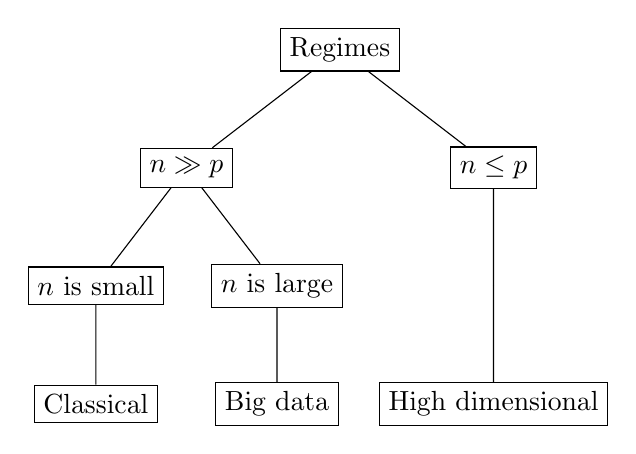
\begin{tikzpicture}
    \tikzstyle{every node}=[rectangle,draw]
    \tikzstyle{level 1}=[sibling distance=39mm] 
    \tikzstyle{level 2}=[sibling distance=23mm]     
    \node {\smallCapGreen{Regimes}}
        child { node {$n \gg p$}
            child { node {\alb{$n$ is small}}
            	child { node {\alb{Classical}}}
            }
            child { node {\alo{$n$ is large}} 
           	child { node {\alo{Big data}} } 	
	  }
        }
        child { node {\alr{$n \leq p$}}
                	   child { %node {\alr{High dimensional} }
        	   child { node {\alr{High dimensional} }}
	   }
        }
         ;
\end{tikzpicture}
\end{center}

\end{frame}

\begin{frame}
\frametitle{Classical regime}
Suppose we have the matrix $\X$ with the features we're considering

\vsp
Now, we want to estimate a parameter vector $\beta$ in the model
\[
Y = \X\beta + \epsilon
\]
\script{E.g. we are modeling the \alo{regression function} as (globally) linear in these features}

\vsp
Minimize the training error $\hat{R}(f)$ over all functions $f_\beta(X) = X^{\top}\beta$
\[
\hat\beta_{LS} = \argmin_\beta \hat{R}(f_\beta) = \argmin_\beta \norm{Y - \X\beta}_2^2
\]
\script{Though we write this as equality, there is only a unique solution if $\textrm{rank}(\X) = p$}
\end{frame}

\begin{frame}
\frametitle{Classical regime}

\vsp
In this case, 
\[
\hat{f}(X) = X^{\top} \hat\beta_{LS} 
= 
X^{\top} \X^{\dagger}Y 
\underbrace{=}_{\textrm{rank}(\X) = p} 
X^{\top}(\X^{\top} \X)^{-1} \X^{\top} Y
\]
\script{$\X^{\dagger}$ is the Moore-Penrose pseudo inverse}
\vsp

The fitted values are $\X\hat\beta_{LS} = H Y$, where $H$ is the orthogonal projection onto the 
column space of $\X$

\script{Contrary to $\hat\beta_{LS}$, the fitted values are always unique}
\end{frame}


%\begin{frame}
%\frametitle{Low-dimensional linear regression ($K \leq n$)}
%Supposing that the functions $\phi_k$ are {\it known}, 
%we can form the \alg{least-squares estimator} by
%``plugging in'' the empirical measure for the unknown true measure
%\[
%\hat{f}= \argmin_{f \in \Phi} \hat{\P}\ell_f,
%\]
%where, for each  $f \in \Phi$, there is a coefficient vector $\beta$ such that 
%$\ell_f(Z) = (X^{\top}\beta - Y)^2$.
%\vsp
%
%In this case, 
%\[
%\hat{f}(X) = X^{\top} \hat \beta,
%\]
%where 
%\[
%\hat\beta = \X^{\dagger}Y = (\X^{\top} \X)^{-1} \X^{\top} Y
%\]
%and $\X^{\dagger}$ is the Moore-Penrose pseudo inverse\note.
%
%\vsp
%In particular, the fitted values are $\X\hat\beta = H Y$, where $H$ is the orthogonal projection onto the 
%column space of $\X$
%\end{frame}
%\begin{frame}
%\frametitle{Classical regime}
%\end{frame}


\begin{frame}
\frametitle{Classical regime}
We can examine the first and second moment properties of $\hat\beta_{LS}$

\begin{align}
\label{eq:bias}
\E \hat\beta_{LS}  & =  \beta \qquad (\textrm{unbiased})\\
\label{eq:var}
\V \hat\beta_{LS}  & =  \X^{\dagger} (\V Y) (\X^{\dagger})^{\top}  
\underbrace{=}_{\textrm{rank}(\X) = p, \V Y \propto I_n} 
 \V[Y_i] (\X^{\top}\X)^{-1} 
\end{align}

\smallCapGreen{Note:} Here is where we need to be more careful:

\vsp
The `true' parameter $\beta$ we are estimating is a coefficient vector of 
the linear oracle with respect
to 
\[
\{ f: \textrm{ There exists } \beta \textrm{ where } f(X) = \beta^\top X\}
\]

\vsp 
There is no reason to believe this approximation error is zero, hence `bias' really references
the linear oracle
\end{frame}

\begin{frame}
\frametitle{Classical regime}

The Gauss-Markov theorem assures us that this is the best linear \alo{unbiased} estimator of $\beta$

\script{Effectively, equation (\ref{eq:var}) is minimized subject to equation (\ref{eq:bias})}

\vsp
Also, it is the maximum likelihood estimator under a homoskedastic, independent Gaussian model

\script{Hence, it is asymptotically efficient}
\vsp

Does that necessarily mean it is any good?
\end{frame}
%
%\begin{frame}
%\frametitle{Low-dimensional linear regression ($K \leq n$)}
%We can examine the first and second moment properties of $\hat\beta$
%
%Focusing on the $f_{*,\Phi} = \beta^{\top}\Phi$ component\footnote{This is important! In claiming $\hat\beta$ is 
%`unbiased' we are asserting either that: (1)  $f_{*,\Phi^c} \equiv 0$ or (2) it is unbiased for the coefficients of
%the linear oracle $f_{*,\Phi}$.} 
%\begin{align}
%\label{eq:bias}
%\E \hat\beta  & =  \beta \qquad (\textrm{unbiased})\\
%\label{eq:var}
%\V \hat\beta  & =  \X^{\dagger} (\V Y) (\X^{\dagger})^{\top}  = \V[Y_i] (\X^{\top}\X)^{-1} 
%\end{align}
%
%The Gauss-Markov theorem assures us that this is the best linear \alo{unbiased} estimator of $\beta$
%
%\script{That is, equation (\ref{eq:var}) is minimized subject to equation (\ref{eq:bias})}
%
%\vsp
%Also, it is the maximum likelihood estimator under a homoskedastic, independent Gaussian model
%
%\script{Hence, it is asymptotically efficient}
%\vsp
%
%Does that necessarily mean it is any good?
%\end{frame}


\begin{frame}
\frametitle{Classical regime}
Write $\X = U D V^{\top}$ for the SVD of $\X$
\vsp

Then $\V \hat\beta_{LS}  \propto (\X^{\top}\X)^{-1}  
= 
VD^{-1}\underbrace{U^{\top}U}_{=I} D^{-1} V^{\top}
=
VD^{-2}  V^{\top}$
\vsp

\smallCapGreen{Reminder:} Elements of $D$, $d_j$, are the axes lengths of the ellipse induced by $\X$
\vsp

Also, suppose we are interested in estimating $\beta$,
\[
\E|| \hat\beta_{LS} - \beta||_2^2  =  \textrm{trace}(\V\hat\beta) \propto \sum_{j=1}^p \frac{1}{d_j^2}
\]
\script{Can you show this? Hint: add and subtract $\E\hat\beta_{LS}$}
\vsp

\smallCapGreen{Important:} Even in the classical regime, we can do arbitrarily badly if $d_p \approx 0$!
\end{frame}


\begin{frame}
\frametitle{Returning to polynomial example: Bias}
\begin{figure}
\centering
  \includegraphics[width=1.65in,trim=0 15 0 20,clip]{../figures/polynomialExample.pdf}
\end{figure}

Using a Taylor's series, for all $X$
\[
\sin(X) = \sum_{q = 0}^\infty \frac{(-1)^qX^{2q+1}}{(2q + 1)!}  = \Phi(X)^{\top}\beta
\]
Higher order polynomial models will \alo{reduce} the bias part
\end{frame}
\begin{frame}
\frametitle{Returning to polynomial example: Variance}
The least squares solution is given by solving $\min \norm{\X\beta - Y}_2^2$

\[
\X =
\begin{bmatrix}
1 & X_1 & \ldots & X_1^{p-1} \\
   & \vdots && \\
 1 & X_n & \ldots & X_n^{p-1} \\
\end{bmatrix},
\]
is the associated Vandermonde\Note matrix. 

\vsp
This matrix is well known for being numerically unstable

\vsp
\script{Letting $\X = UDV^{\top}$, this means that $d_1/d_p \rightarrow \infty$} 

\vsp 
Hence\footnote{This should be compared with the variance computation in equation (\ref{eq:var})}
\[
||(\X^{\top}\X)^{-1}||_2 = \frac{1}{d_p^2}
\]
grows larger, where here $||\cdot||_2$ is the \alg{spectral (operator) norm}\Note
\end{frame}

\begin{frame}
\frametitle{Returning to the polynomial example}
\begin{figure}
\centering
  \includegraphics[width=2.5in,trim=0 15 0 20,clip]{../figures/polynomialExample.pdf}
\end{figure}
\end{frame}


\begin{frame}
\frametitle{Conclusion}
\smallCapGreen{Conclusion:} Fitting the full least squares model, even in the classical regime,
can lead to poor prediction/estimation performance

\vsp
In the other regimes, we encounter even for sinister problems
\end{frame}


\begin{frame}
\frametitle{Big data regime}
\alo{Big data}: The computational complexity scales extremely quickly.  This means that 
procedures that are feasible classically are not for large data sets

\vsp
\smallCapGreen{Example:} Fit $\hat\beta_{LS}$ with $\X \in \R^{ n \times p}$.  Next 
fit $\hat\beta_{LS}$ with $\X \in \R^{ 3n \times 4p}$

\vsp
The second case will take $\approx$ $(3*4^2) = 48$ times longer to compute, as well as 
$\approx 12$ times as much memory!

\script{Actually, for software such as \alr{R} it might take 36 times as much memory, though there are data structures
specifically engineered for this purpose that update objects `in place'}
\end{frame}

\begin{frame}[fragile]
\frametitle{Conclusion}
\begin{blockcode}
p = 300; n = 10000
Y = rnorm(n); X = matrix(rnorm(n*p),nrow=n,ncol=p)
start = proc.time()[3]
out   = lm(Y~.,data=data.frame(X))
end   = proc.time()[3]
smallTime = end - start

n = nMultiple*n; nMultiple = 3
p = pMultiple*p; pMultiple = 4
Y = rnorm(n); X = matrix(rnorm(n*p),nrow=n,ncol=p)
start = proc.time()[3]
out   = lm(Y~.,data=data.frame(X))
end   = proc.time()[3]
bigTime = end - start
> print(bigTime/smallTime)
 elapsed 
38.61458 
> print(nMultiple*pMultiple**2)
[1] 48
\end{blockcode}
\end{frame}

\begin{frame}
\frametitle{Example big data problem}
\begin{figure}[h]
   \centering
   \includegraphics[width=4.75in]{../figures/watsonEbayAuction} % requires the graphicx package
\end{figure}


\end{frame}


\begin{frame}
\frametitle{Example big data problem}
Buyer:
\vspace{-.3in}
\begin{figure}[h]
   \centering
   \includegraphics[width=4.65in]{../figures/watsonEbayCommentBuyer}\\
\end{figure}
\vsp

Seller:
\vspace{-.3in}
\begin{figure}[h]
   \centering
   \includegraphics[width=4.65in]{../figures/watsonEbayCommentSeller}
\end{figure}

\vvsp

The data ($\sim$750 Gb, millions of rows, thousands of columns):
\vvvsp

\tiny
\begin{tabular}{llllllllllllllllll}
  User & ID & Rating                &                     Comment & Role & WinBid &    SellerID  \\
 dorkyporky           &        134    &  1 & fast delivery.....very good seller...AAA++     &      B  &15.51&princesskitten2001
\end{tabular}

\end{frame}
%
%
%\begin{frame}[fragile]
%\frametitle{Conclusion}
%\smallCapGreen{Example:} 
%\end{frame}

\begin{frame}
\frametitle{High dimensional regime}
 \alr{High dimensional}: These problems tend to have many of the computational problems 
as \alo{Big data}, as well as a \alg{rank problem}:

\vsp
Suppose $\X \in \R^{n \times p}$ and $p > n$

\vsp
Then $\textrm{rank}(\X) = n$ and the equation $\X\hat{\beta} = Y$:
\begin{itemize}
\item can be solved \emph{exactly} (that is; the training error is 0)
\item has an infinite number of solutions
\end{itemize}

\begin{table}
   \centering
   \begin{tabular}{cc}
   \includegraphics[width=1.55in]{../figures/introLinearModelConvexStrict.pdf} &
      \includegraphics[width=1.55in]{../figures/introLinearModelConvexNotStrict.pdf} \\
      $n > p$ & $n < p$ 
      \end{tabular}
\end{table}
\end{frame}

\begin{frame}
\frametitle{High dimensional regime: Example}
\begin{figure}
\centering
   \includegraphics[width=1.35in]{../figures/highDimensionalExample.pdf} 
\end{figure}
\end{frame}
\end{document}
